\section{Управление рисками предприятия, методы оценки рисков}

Управление рисками --- это процессы, связанные с идентификацией, анализом рисков и принятием решений, которые включают максимизацию положительных и минимизацию отрицательных последствий наступления рисковых событий. Процесс управления рисками проекта обычно включает выполнение процедур, приведенных на рисунке \ref{fig:diagram-page-2}.

\begin{figure}[!h]
	\centering
	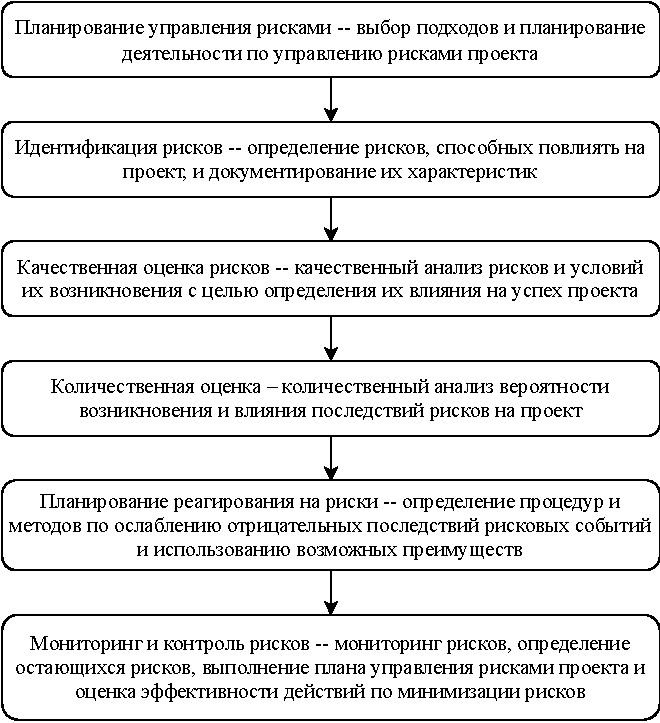
\includegraphics[width=0.7\linewidth]{Diagram-Page-2}
	\caption{Этапы управления рисками проекта}
	\label{fig:diagram-page-2}
\end{figure}

Планирование управления рисками --- процесс принятия решений по применению и планированию управления рисками для конкретного проекта. Этот процесс может включать в себя решения по организации, кадровому обеспечению процедур управления рисками проекта, выбор предпочтительной методологии, источников данных для идентификации риска, временной интервал для анализа ситуации. Важно спланировать управление рисками, адекватное как уровню и типу риска, так и важности проекта для организации.

Идентификация рисков --- заключается в систематическом выявлении рисков, характерных для определенного вида деятельности, и определении их характеристик.

Идентификация сводится к выявлению возможных проблем. 
Под «проблемой» понимают что-либо (событие, объект, человека, идею), что может встать между организацией и ее целями.
Необходимо определить, что пойдет «не так», чтобы затем решить, как это устранить или обойти.

Идентификация риска --- процесс нахождения, составления перечня и описания элементов риска.
Основные элементы риска:
\begin{itemize}
\item  причины, приводящие к наступлению опасного явления;
\item опасные явления (события), оказывающие воздействие на объект;
\item виды воздействия, которые могут привести к изменению состояния объекта;
\item последствия, представляющие собой потери из-за воздействия, и их оценку со стороны субъекта;
\item факторы риска, влияющие на вероятность реализации риска и тяжесть последствий.
\end{itemize}

Качественная оценка рисков – процесс представления качественного анализа
идентификации рисков и определения рисков, требующих быстрого реагирования. Такая
оценка рисков определяет степень важности риска и выбирает способ реагирования.
Доступность сопровождающей информации помогает легче расставить приоритеты для
разных категорий рисков. Качественная оценка рисков это оценка условий возникновения
рисков и определение их воздействия на проект стандартными методами и средствами.
Использование этих средств помогает частично избежать неопределенности, которые
часто встречаются в проекте. В течение жизненного цикла проекта должна происходить
постоянная переоценка рисков.

Количественная оценка рисков определяет вероятность возникновения рисков и
влияние последствий рисков на проект, что помогает группе управления проектами верно
принимать решения и избегать неопределенностей. Количественная оценка рисков
позволяет определять:
- вероятность достижения конечной цели проекта,
- степень воздействия риска на проект и объемы непредвиденных затрат и
материалов, которые могут понадобиться,
- риски, требующие скорейшего реагирования и большего внимания, а также
влияние их последствий на проект,
- фактические затраты, предполагаемые сроки окончания.
Количественная оценка рисков часто сопровождает качественную оценку и также
требует процесс идентификации рисков. Количественная и количественная оценка рисков
могут использоваться по отдельности или вместе, в зависимости от располагаемого
времени и бюджета, необходимости в количественной или качественной оценке рисков.

Планирование реагирования на риски - это разработка методов и технологий
снижения отрицательного воздействия рисков на проект. Берет на себя ответственность за
эффективность защиты проекта от воздействия на него рисков. Планирование включает в
себя идентификацию и распределение каждого риска по категориям. Эффективность
разработки реагирования прямо определит, будут ли последствия воздействие риска на
проект положительными или отрицательными.
Стратегия планирования реагирования должна соответствовать типам рисков,
рентабельности ресурсов и временным параметрам. Вопросы, обсуждаемые во время
встреч, должны быть адекватны задачам на каждой стадии проекта, и согласованы со
всеми членами группы по управлению проектом. Обычно требуются несколько вариантов
стратегий реагирования на риски.

Мониторинг и контроль следят за идентификацией рисков, определяют
остаточные риски, обеспечивают выполнение плана рисков и оценивают его
эффективность с учетом понижения риска. Показатели рисков, связанные с
осуществлением условий выполнения плана фиксируются. Мониторинг и контроль
сопровождает процесс внедрения проекта в жизнь.
Качественный контроль выполнения проекта предоставляет информацию,
помогающую принимать эффективные решения для предотвращения возникновений
рисков. Для предоставления полной информации о выполнении проекта необходимо
взаимодействие между всеми менеджерами проекта.
Целью мониторинга и контроля является выяснить, было ли:
- Система реагирования на риски внедрена в соответствии с планом
- Реагирование достаточно эффективно или необходимы изменения
- Риски изменились по сравнению с предыдущим значением
- Наступление влияния рисков
- Необходимые меры приняты
- Воздействие рисков оказалось запланированным или явилось случайным
результатом.
Контроль может повлечь за собой выбор альтернативных стратегий, принятие
корректив, перепланировку проекта для достижения базового плана. Между менеджерами
проекта и группой риска должно быть постоянное взаимодействие, должны
фиксироваться все изменения и явления. Отчеты по выполнению проекта должны
формироваться регулярно.
Можно более подробно рассмотреть риск-менеджмент, который включает
алгоритм выбора таких инструментов (в том числе страховой услуги и конкретного
страховщика) для решения задач обеспечения бесперебойности реализуемого имвоспроизводственного процесса или его части. Известно, что алгоритмом называют
однозначную последовательность действий.
Для того, чтобы выбрать один из альтернативных инструментов и вариантов
действий может быть предложен следующий алгоритм риск-менеджмента:
1) сформулировать цель действий;
2) синтезировать критерий - правило выбора наилучшего варианта действий из
ряда возможных;
3) провести анализ внешней среды, в которой проводится операция или работает
системы с целью выделения возможных источников риска',
4) провести анализ разрабатываемой операции или системы с целью выделения
возможных источников риска (баллоны с горюче-смазочными, взрывчатыми и химически
вредными веществами; элементы конструкции, которые могут сорваться, и т.п.);
5) провести анализ внешней среды, в которой проводится операция или работает
система с целью выделения объектов, уязвимых по отношению к поражающим факторам,
которые могут возникнуть при реализации источников риска;
6) оценить частоту появления источника риска для отдельных элементов системы
и(или) операции. На основе этой информации составить перечень наиболее вероятных
страховых случаев (пожар, кража и т.д.);
7) разработать прогноз - оценить вероятность страхового случая и средний
возможный ущерб при каждом из страховых случаев;
8) оценить материальные затраты на то, чтобы предупредить (исключить
возможность реализации или снизить вероятность) возможность реализации риска;
9) используя критерий, провести рациональное распределение и(или)
оптимизировать распределение средств между мероприятиями:
- по устранению источника риска;
- по снижению риска посредством уменьшения интенсивности поражающих
факторов или уязвимости объектов, которые могут подвергнуться воздействию
поражающих факторов;
- по компенсации ущерба (последствий) риска (В этом случае заключают договор
страхования. При наступлении страхового случая и возникновении ущерба его
компенсируют за счет сумм, полученных по страховке.);
10) оценить уровень безопасности и достаточность принятых мер. А если будет
признана недостаточность мер по предупреждению и снижению рисков, то оценить
располагаемые остаточные финансовые ресурсы, которые могут быть направлены на
страхование;
11) если окажется более целесообразным страхование, то вначале необходимо
оценить возможность использования в условиях конкретной операции нефондового
страхования.
Выбор формы страхования (нефондовое или фондовое страхование) определяется
характером операции, ситуацией на финансовом или товарном рынке, располагаемыми
финансовыми ресурсами.
Впрочем всегда существует стремление использовать нефондовое страхование,
позволяющее более гибко реагировать на рыночную ситуацию, включив неявный
"страховой взнос" в цену, и заплатить этот взнос не до начала проекта (как то происходит
при фондовом страховании), а при первичном распределении цены товара или
финансового инструмента. Поэтому практически традиционное фондовое страхование
применяется только тогда, когда характер операции, рыночная ситуация не позволяют
использовать нефондовое страхование, и когда имеются ранее накопленные финансовые
ресурсы. Важно, что источником формирования страхового фонда является добавочное
производство. Это связано с тем, что в условиях простого воспроизводства отсутствует
возможность для выделения запасов.Источником страхового фонда может быть и часть необходимого продукта. Так
формируют фонды обязательного страхования: пенсионный фонд, фонд занятости, фонд
медицинского страхования, обязательного социального страхования.
12) в противном случае (использовать нефондовое страхование невозможно)
оценить рациональную цену страховой услуги. Для этого страхователь должен сам
оценить возможный ущерб от реализации источников риска с учетом вероятности
появления соответствующих страховых случаев. При этом страхователь может (например,
с помощью экспертных методов или описанного выше статистического имитационного
моделирования) прогнозировать:
- вероятность наступления страхового случая;
- математическое ожидание величины ущерба при наступлении страхового случая;
- убыточности страховой суммы как произведение вероятности наступления
страхового случая и математического ожидания величины ущерба;
- нетто-ставку страхового тарифа (например, приравняв ее убыточности) по
отношению к конкретному виду страхования.
- брутто-ставку.
Из практики страховой деятельности в РФ известно, что нетто-ставка составляет
(60-70)% брутто-ставки (равной цене страховой услуги). Таким образом страхователь
может самостоятельно оценить рациональную величину страховой премии;
13) выбрать страховщика - страховую организацию для заключения договора
страхования с учетом размера собственного капитала страховщика, деловой репутации,
цены услуги, результатов аудита деятельности этой страховой компании за
предшествующий период и всей другой доступной информации.
Основной задачей предлагаемой методики оценки рисков является их
систематизация и разработка комплексного подхода к определению степени риска,
влияющего на финансово-хозяйственную деятельность предприятия. Предлагается
следующий алгоритм оценки рисков, который приведен на рис. 2.5.















